\scanpage{181}
\mspage{90}

d'isomorphie d'un tel torseur s'identifie d'ailleurs, par la suite exacte de coh. \unsure{associé} à la suite exacte
\[
0 \longrightarrow \pi \longrightarrow
\pi\otimes_{\mathbb Z}\unsure{\mathbb C|\mathbb R}
\longrightarrow U_0 \longrightarrow 0
\]
\inserted{ou \(\pi\otimes_{\mathbb Z}\mathbb R\)}
à une classe d'extensions de \(\Gamma\) par \(\pi\).
Mais dire que l'action de \(\Gamma\) sur \(\pi\) est triviale, signifie que l'action de \(\Gamma\) sur le torseur \(U\) sous \(U_0\) se fait par translations.

\inserted{\uuline{Corollaire-scholie}}
\uline{\unsure{NB}} Le cas ``abélien'' n'est pas tout à fait démontré, faute d'avoir établi la \deleted{\unsure{top.}} classification \inserted{top.} des opérations d'un groupe fini sur \(\mathbb C^{*}\) ou sur \(S^1\times S^1\). Cependant si dans le cas abélien on suppose d'avance que \(U^\Gamma\ne\varnothing\), \uline{alors} \deleted{les conditions a) b) \unsure{c)}} il est encore vrai que l'opération triviale de \(\Gamma\) sur \(\pi\) équivaut à la trivialité de l'action de \(\Gamma\) sur \(U\). Car on est ramené au cas où \(\Gamma\) opère fidèlement, et à prouver dans ce cas que si l'op. de \(\Gamma\) sur le \(\pi\) est triviale, on a \(\Gamma=1\). Et on fait comme plus haut dans le cas anabélien.

\scanpage{182}
\mspage{91}

\deleted{\unsure{Supplément|Supprimé}}
\uline{18} \uline{Forage de trous.} Application aux actions extérieures de groupes finis

Soit \(\Pi'\) un groupe à lacets de type \((g,\nu+1)\)\inserted{\(\unsure{(\nu+1\in\mathbb N^*)|(\nu\in\mathbb N^*)}\)}, non abélien i.e. \deleted{\(g\ge2\) ou \(g=1,\nu\ge1\) ou} \inserted{\deleted{\illegible{1}}, \unsure{si}} \(g=0\), \inserted{\unsure{on a}} \(\nu\ge2\)
\deleted{(i.e. \(2g+\unsure{\nu\geq2}\quad 2g+\nu\ge\unsure{2|3}\) i.e. \(\deleted{\illegible{1}}2-2g\,(=\mathrm{EP})\le\nu\)).}
Soient \(T\) son module des orientations, et \(I'\) \((\operatorname{card}I'=\unsure{\nu})\) l'ens. de ses classes de conjugaison de ss-groupes de lacets. Fixons nous un \(i\in I'\), et soit \(L'_i\subset\Pi'\) dans la classe \(i\).

Quand on se donne \deleted{\(\Pi'\) en tant que} \inserted{seulement un} groupe \uline{extérieur} \deleted{\illegible{1}}\inserted{à lacets \(\unsure{[\Pi']}\)} (ce qui \deleted{\unsure{est fait}} équivaut à la donnée de \(B_{D'^*}\longrightarrow B_{U'}\)), la donnée d'un \deleted{\illegible{1}} \(i\in I'\) équivaut à celle d'une comp. connexe de \(B_{D'^*}\), et celle d'une réalisation \deleted{\unsure{\((L_i,\Pi)\)}} du groupe cat. (i.e d'un couple d'un groupe \(\Pi'_{\unsure{s|\alpha}}\), et d'un isom. cat. \(\Pi'\longrightarrow[\Pi']_{\unsure{d}}\)) \inserted{équivaut à isom unique près} \deleted{\illegible{3}}\inserted{(rev. universel \(\widetilde U'\) de \(U'\), par \(\Pi'=\operatorname{Aut}(\widetilde U')\).} de \(\Pi_1B_{U'}\), Enfin la donnée d'un couple \((\Pi',L_i')\) (\(L_i'\) dans la classe de conjugaison \(i\)) équivaut \inserted{(à isom unique près)} à la donnée \unsure{d'un} objt \inserted{\(\widetilde D_i^{\unsure{*}}\)} de \(\Pi_1B_{D_i'^*}\) -- on prend l'image \(\widetilde U'\) de \(\widetilde D^{*'}\) dans \(\Pi_1B_{U'}\), et
\[
\Pi'=\operatorname{Aut}(\widetilde U'),\qquad
L'_i=\operatorname{Im}\bigl(\operatorname{Aut}(\widetilde D_i'^*)\longrightarrow
\operatorname{Aut}(\widetilde U')\bigr).
\]
\margin{\unsure{Je vais} provisoirement \unsure{laisser tomber} les ``primes'' !}

Quand on se donne \deleted{une réalisation} \inserted{\unsure{d'origine|d'où une}} un objt \(\widetilde U'_0\) de \(\Pi_1B_{U'}\), \unsure{d'où} \inserted{\(\Pi'=\operatorname{Aut}(\widetilde U'_0)\)}, alors

\scanpage{183}

la donnée d'un \(L_i\subset\pi\) dans la classe \(i\) équivaut à la donnée d'un couple \((\widetilde D_i,\unsure{\lambda|\operatorname{id}})\) d'un \(\widetilde D_i\in\operatorname{Ob}\Pi_1B_{D_i}\) et d'un isom de \(\rho_!(\widetilde D_i)\unsure{=:|=}\widetilde U\) sur \(\widetilde U_0\).

Quand \deleted{\(\pi\) est réalisé} la situation toposique est réalisée à partir d'une situation topologique \((X,S)\), et qu'on définit \(\widetilde U_0\) à l'aide d'un pt base \(a\in U\), alors la façon standard de définir un \(L_i\subset\pi=\operatorname{Aut}(\widetilde U_0)=\pi_1(U,a)\) est de choisir une petite \unsure{rondelle} \(\Delta_i\) autour de \(s_i\) dans \(X\),
\figure{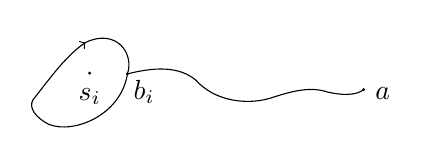
\begin{tikzpicture}[x=1cm,y=1cm,line cap=round,line join=round,baseline=(current bounding box.center)]
\coordinate (b) at (0.48,0.15);
\coordinate (a) at (3.48,-0.05);
\draw[->] (-0.72,-0.18) .. controls (-0.50,0.10) and (-0.30,0.38) .. (-0.05,0.55);
\draw (-0.05,0.55) .. controls (0.33,0.73) and (0.57,0.42) .. (b)
  .. controls (0.40,-0.37) and (-0.20,-0.62) .. (-0.52,-0.49)
  .. controls (-0.68,-0.41) and (-0.78,-0.28) .. (-0.72,-0.18);
\fill (0,0.16) circle (0.6pt);
\node[below] at (0,0.09) {$s_i$};
\fill (b) circle (0.6pt);
\node[below right,inner sep=2pt] at (b) {$b_i$};
\draw (b) .. controls (0.80,0.23) and (1.12,0.26) .. (1.35,0.07)
  .. controls (1.58,-0.19) and (1.98,-0.25) .. (2.29,-0.16)
  .. controls (2.59,-0.06) and (2.81,-0.01) .. (3.02,-0.08)
  .. controls (3.19,-0.12) and (3.38,-0.13) .. (a);
\fill (a) circle (0.6pt);
\node[right,inner sep=4pt] at (3.48,-0.10) {$a$};
\end{tikzpicture}}
et un pt \inserted{\(b_i\)} sur le bord, et une classe d'homotopie de chemins \inserted{(dans \(\deleted{\unsure{X}}\unsure{U|X}-(\mathring\Delta_i-\{s_i\})=V_i\))} de \(a\) vers \(b_i\), et de prendre le groupe \(L_i\) engendré par l'un quelconque des deux lacets correspondants autour de \(s_i\) (qui donnent des \deleted{\unsure{deux}} élts opposés de \(\pi\)).
On voit que l'on trouve ainsi une application surjective de
\[
\operatorname{Isom}_{\Pi_1V_i}(a,b_i)\simeq
\operatorname{Isom}_{\Pi_1U}(a,b_i)
\]
\deleted{vers} sur l'ens des \(L_i\subset\pi\) dans la classe \(\unsure{i|\Pi}\), application \deleted{dont} compatible avec l'action

\scanpage{184}
\mspage{92}

naturelle de \(\pi\) (opérant sur \(\operatorname{Isom}_{\Pi_1U}(a,b_i)\) de la façon évidente par composition, et sur l'ens des \(L_i\) par autom. int.
\deleted{\unsure{Alors}} Ici, le \deleted{choix de} lien avec la description ``abstraite'' toposique s'établit ainsi: le choix de \(b_i\) peut servir de pt \unsure{base|fixe} pour définir un rev. universel de \(\Delta_i\smallsetminus\{s_i\}\overset{\sim}{\hookleftarrow}D_i^*\), d'où un objt \(\rho_!(\widetilde D_i^*(b_i))\), et \deleted{\unsure{cet objt}} les \(L_i\subset\pi\) correspondent \inserted{(d'après la description abstraite)} aux isom de \(\widetilde U_0=\widetilde U(a_i)\) sur \(\unsure{D_i^*(b_i)|\widetilde D_i^*(b_i)}\) modulo composition avec un autom de \(\unsure{D_i^*(b_i)|\widetilde D_i^*(b_i)}\) provenant d'un autom de \(\unsure{D_i^*(b_i)|\widetilde D_i^*(b_i)}\) -- mais les iso \deleted{de} \(\widetilde U(a_i)\xrightarrow{\sim}\rho_!(\widetilde D_i^*(b_i))\) correspondent justement aux classes de chemins de \(a\) vers \(b_i\).

\margin{On revient aux notations \(\pi',U'\) --}
\unsure{Considérons} un objt de \(\Pi_1B_{D_i^{*'}}\), i.e. un couple \((\pi',L_i')\). Soit \(\pi\) le groupe quotient de \(\pi'\) par le ss-groupe invariant de \(\pi'\) \deleted{défini} \inserted{engendré} par \(L_i'\). Je dis \margin{\(\Vert\)} qu'à isom unique près (isom effectif de groupes, pas seulement extérieur !) il ne

\scanpage{185}

dépend pas du choix de l'objt \(\widetilde D_i^*\) de \(\Pi_1B_{D_i'^*}\). En effet, \(\pi=\pi(\widetilde D_i^*)\) dépend fonctoriellement de \(\widetilde D_i^*\), et tt revient à voir que ce foncteur est \uline{constant}, i.e. que l'opération de
\[
\operatorname{Aut}(\widetilde D_i^*)\simeq T\simeq L_i
\quad\text{sur}\quad
\pi=\pi(\widetilde D_i^*)
\]
est triviale. Or soit \(u\in L_i\), \unsure{l'|son} autom de \(\pi\) qu'il définit est défini par l'autom. intérieur \(\operatorname{int}(u)\) par passage au quotient, donc (comme \(u\) devient \(1\) dans \(\pi\)) il est trivial. \unsure{Facile.}

On trouve ainsi un \uline{foncteur}
\[
\begin{array}{c}
\text{Groupes extérieurs à lacets }\pi'\\
\text{de type }g,\nu+1\text{ munis d'une}\\
\text{classe de lacets }i\in I(\pi')
\end{array}
\longrightarrow
\begin{array}{c}
\text{groupes}\\
\text{(réalisés)}\\
\text{à lacets, de}\\
\text{type }g,\nu\deleted{\unsure{+1}}
\end{array}
\]
\[
(\pi',i)\longmapsto\beta(\pi',i)
\qquad
\text{[``bouchage du trou \(i\)'']}
\]
qui s'exprime par un hom de groupes
\[
\operatorname{Aut\,ext}(\pi',i)\longrightarrow\operatorname{Aut}\pi
\tag{\unsure{*|5}}
\]
où \(\pi=\beta(\pi',i)\)
\[
\left(
\begin{array}{l}
\overset{\text{déf}}{=}\text{ ens. des autom cat.}\\
\text{de }\pi'\text{ respectant la structure}\\
\text{à lacets et fixant la classe de}\\
\text{lacets }i
\end{array}
\right)
\]

\scanpage{186}
\mspage{93}

Du point de vue géométrique, ce fait (existence de ce foncteur), ne fait qu'exprimer le fait qu'après ``bouchage du trou'' \(i\), on a un \deleted{pt.} \(U=U'\cup\{s_i\}\) \uline{muni} d'un pt \(s_i\) qu'on peut utiliser comme un \uline{pt base} \inserted{\uuline{canonique}} pour calculer \(\pi_1(U)\).

On peut dire aussi que le choix de \(i\) permet de construire la somme amalgamée partielle (bouchage de trous \inserted{partiel}) \(B_{U^*}\)
\diagram{
\begin{tikzcd}[ampersand replacement=\&]
\& B_{D_i'^*} \arrow[dl] \arrow[dr] \& \\
B_{U'} \arrow[dr] \& \& B_{s_i} \arrow[dl] \\
\& B_{U^*} \&
\end{tikzcd}
}
et \(B_{s_i}\longrightarrow B_{U^*}\) fournit un pt géom. de \(B_{U^*}\) qui permet de décrire un objt canonique de \(\Pi_1B_{U^*}\) (rev universel relatif à ce pt) d'où canoniquement un groupe \(\pi\), qui bien sûr est un groupe à lacets de type \(g,\nu-1\).

\uline{Théorème} Supposons \(g,\nu\) tels que non

\scanpage{187}

seulement les groupes \(\pi'_{\unsure{s}}\) de type \(g,\nu\), mais aussi les groupes \(\pi\) (de type \(g,\nu-1\)) soient anabéliens, i.e.
\[
2g+\unsure{\nu}\deleted{\unsure{+1}}\unsure{\ge|\le}\unsure{4}
\quad
[\text{donc }g\ge2,\ \text{ou }g\unsure{\ge|=}1,\nu\ge2,\ \text{ou }g=0,\nu\ge4].
\]
Alors le foncteur précédent \((\pi',i)\longrightarrow\pi\) est une équivalence de catégories, en d'autres termes (comme il s'agit de groupoïdes \(0\)-connexes)
\[
\operatorname{Aut\,ext}(\pi',i)\longrightarrow\operatorname{Aut}(\pi)
\]
est un \uline{isomorphisme}.

Notons pour ceci \unsure{qu'on a} la suite exacte
\[
1\longrightarrow\pi\longrightarrow\operatorname{Aut}(\pi)
\longrightarrow\operatorname{Aut\,ext}(\pi)\longrightarrow1:
\]
(car \(\operatorname{Centre}\pi=1\) par hyp anabélienne sur \(\pi\)), \unsure{or} on va définir une suite exacte
\[
1\longrightarrow\pi\longrightarrow\operatorname{Aut\,ext}(\pi',i)
\longrightarrow\unsure{\operatorname{Aut\,ext}(\pi)|\operatorname{Aut\,ext}(\pi')}
\longrightarrow1
\]
et un hom. d'extensions de celle-ci

\scanpage{188}
\mspage{\unsure{94|99}}

dans la précédente (qui sera nécessairement un isomorphisme).

OPS \(T=\mathbb Z\), on considère les groupes à lacets \unsure{standart|standard} \(\Pi_{g,\nu+1}\), \(\Pi_{g,\nu}\). Posons
\[
\operatorname{Aut\,ext}_{\mathrm{lac}}(\Pi_{g,\nu})
=\unsure{\mathcal T|\mathfrak T}_{g,\nu}^{\unsure{00|\circ\circ}}
\]
\inserted{induisant \uline{l'identité} sur \(I(\Pi_{g,\nu})\) et sur \(T(\Pi_{g,\nu})\)}
(groupe de Teichmüller d'indice \(g,\nu\)),
on sait que (pour \(2g+\nu\ge3\)) \(\mathcal T_{g,\nu}\) est le groupe fondamental du topos modulaire complexe \inserted{\(M_{g,\nu}\)} des courbes complexes (\deleted{\illegible{1}} \unsure{proj. n.s.}) conn., de genre \(g\), avec un syst de \(\nu\) pts \(s_1-\!s_\nu\) distincts donnés.
\margin{\uline{NB.} le rev. universel de \(M_{g,\nu}\) est contractible, Teichmüller.}
Or le topos modulaire \(M_{g,\nu+1}\) n'est autre que \deleted{l'image} la ``courbe complexe universelle \deleted{\illegible{1}} de genre \(g\) à \(\nu\) trous numérotés'' sur \(M_{g,\nu}\)
[car se donner une courbe \inserted{\(U'\)} de genre \(g\) avec \(\nu+1\) trous \inserted{\(x_1-\!x_{\nu+1}\)} revient au \(\overline{\mathrm m}\) que de s'en donner une \inserted{\(U\)} avec \(\nu\) trous numérotés \(x_1-\!x_\nu\), \uline{plus} un \deleted{trou de} pt de \(U\) \deleted{\unsure{pointé}}), \uline{d'où} une suite exacte d'homotopie
\diagram{
\begin{tikzcd}[ampersand replacement=\&,column sep=small]
\unsure{\pi_2|\Pi_2}(M_{g,\nu},\unsure{\xi})
 \arrow[r] \&
\pi_1(U) \arrow[r] \arrow[d,equal] \&
\pi_1(M_{g,\nu+1}) \arrow[r] \arrow[d,equal] \&
\pi_1(M_{g,\nu}) \arrow[r] \arrow[d,phantom,sloped,"\simeq"] \&
\pi_0(U) \arrow[d,equal] \\
0 \arrow[r] \&
\pi=\Pi_{g,\nu} \arrow[r] \&
\mathcal T^{00}_{g,\nu+1} \arrow[r] \&
\mathcal T^{00}_{g,\nu} \arrow[r] \&
1
\end{tikzcd}
}

\scanpage{189}

d'où \unsure{une} structure d'extension \deleted{annoncée}
\[
1\longrightarrow\Pi_{g,\nu}
\longrightarrow\mathcal T^{00}_{g,\nu+1}
\longrightarrow\mathcal T^{00}_{g,\unsure{\nu}}
\longrightarrow1
\]
qui est (à passage à un sous-groupe d'indice ``\(2\nu!\) près) cette structure d'extension annoncée. \unsure{\&} les vérifications de \uline{compatibilité} sont laissées \ldots.

On a donc un foncteur quasi inverse (défini à isom unique près)
\[
\begin{array}{c}
\text{groupes à lacets}\\
\text{de type }g,\nu\\
(2g+\nu\ge3)
\end{array}
\longrightarrow
\begin{array}{c}
\text{groupes \uline{extérieurs} à}\\
\text{lacets de type }(g,\nu+1),\\
\text{avec une ``classe de}\\
\text{lacets'' distinguée}\\
\text{(couples }(\pi',i\in I(\pi'))\text{)}
\end{array}
\]

\deleted{\unsure{Or}} \unsure{Au} niveau toposique, quand on a un système \(B_{D^*}\longrightarrow B_U\) \inserted{de type \(g,\nu\) \((2g+\nu\ge3)\)}, et un ``pt'' de \(B_U\) i.e un \(\widetilde U\in\operatorname{Ob}\Pi_1B_U\), alors on peut de façon canonique trouver un \(B_{D_i^*}\) (\unsure{\(T\)-gr. poïde} \inserted{connexe}, où \(T\) est le module d'orientation), et un système
\[
B_{D^*}\amalg B_{D_i^*}\longrightarrow B_{U'},
\]
de type \(g,\nu+1\),

\scanpage{190}
\mspage{95}

de façon que \((B_{D^*},B_U,\widetilde U)\) \unsure{s'en déduise} par l'opération de ``bouchage du trou \(D_i^*\)''.

Ces constructions sont si fonctorielles, \margin{\unsure{\(\wedge\)}} qu'elles commutent aux actions de groupes \(\Gamma\). Si un groupe \(\Gamma\) opère sur un groupe à lacets \(\pi_{\deleted{\unsure{g,\nu}}}\) de type \(g,\nu\), (pas seulement extérieurement), alors on en déduit une opération \uline{extérieure} de \(\Gamma\) sur un \(\pi'\) à lacets de type \(g,\nu+1\), qui fixe une classe de lacets privilégiée \(i\in I\).

Mais alors, dans l'extension correspondante
\[
1\longrightarrow\pi'\longrightarrow E'\longrightarrow\Gamma\longrightarrow1,
\]
Choisissons un \(L_i'\subset\pi'\) et soit \(\unsure{\mathcal E_i'|E_i'}\) le normalisateur de \(L_i\) dans \(\unsure{\mathcal E'|E'}\) -- on trouve
\[
1\longrightarrow
\underset{\simeq T}{L_i'}
\longrightarrow\unsure{\mathcal E_i'|E_i'}
\longrightarrow\Gamma\longrightarrow1
\]
